\section{Funktionelle krav}\label{funktionellekrav}
\textit{For at sikre systemets funktionalitet i forhold til ovenstående løsningsstrategi opstilles en række funktionelle krav for det samlede system. Disse krav danner grundlag for efterfølgende indhold i kapitlet. Der opstilles ydermere et blokdiagram for at give et overblik kravene til systemet.}

Formålet med systemet er at udvikle en aktivitetsmåler, som har potentialet til at reducere antallet af inaktive børn. Dette gøres med henblik på at ændre den teknologiske udviklings påvirkning på børns aktivitetsvaner fra inaktivitet til aktivitet. Der ønskes et system som detekterer aktiviteterne gang, løb og cykling, da disse er gængse aktiviteter i et barns hverdag. Detekteringen af disse aktiviteter kan ske gennem et accelerometer og og et gyroskop, hvorefter systemet teoretisk kan adskille gang, løb og cykling. Intensiteten af aktiviteterne registreres igennem puls, da dette giver en indikation af det fysiologiske udbytte, som barnet får ud af en given aktivitet. Det vil være væsentligt at sammenholde puls og tid, da det anbefales, at børn skal være aktive 30 minutter med høj intensitet mindst tre gange om ugen. Derudover er et barns kognitive funktion øget i op til 50 minutter efter 11-20 minutters fysisk aktivitet.

For at systemet har en motiverende effekt på børn, skal der være en brugerflade, som børnene finder interessant. Denne skal visuelt give feedback på dagens samlede præstationer samt progressionen i aktivitetsniveauet. Dette gøres, da intensiteten af en aktivitet er essentiel for udbyttet, hvilket beskrives i \secref{subsub:ak_int}. % Børnene udfordres dermed på intensiteten, hvilken kan variere for det enkelte barn ved den samme aktivitet.
Børnene bliver belønnet med point afhængigt af, hvilken aktivitet der udføres og intensiteten heraf.  

Systemet skal være i stand til at detektere børns aktivitet igennem en hel dag uden at være til gene. %, hvormed det skal fungere uafhængigt af andre systemer. 
Det skal dermed være et trådløst system, som kan sende data til en ekstern enhed med faste intervaller og er batteridrevet. Derudover skal det være elektrisk sikkert, således barnet ikke bliver skadet som følge af aktivitetsmålerens design. 

På baggrund af ovenstående udformes de funktionelle krav således, at systemet skal: 
\begin{itemize}
	\item Kunne detektere aktiviteterne gang, løb og cykling gennem bestemte sensorer.
	\item Kunne adskille gang, løb og cykling ved hjælp af algoritmer i softwaren 
	\item Kunne registrere intensiteten af de givne aktiviteter igennem pulssensor.
	\item Være komfortabelt, hvorfor det trådløst skal videresende signaler til en ekstern enhed og være batteridrevet en hel dag.
	\item Være elektrisk sikkert for brugeren.
	\item Behandle og repræsentere signalerne visuelt som intensiteten af en aktivitet i forhold til tid.
	\item Motivere børn i aldersgruppen 9-12 år. 
\end{itemize}

\subsection{Blokdiagram}
Ud fra kravene til systemet udformes et blokdiagram, som illustreres på \figref{fig:blokdiagram}. På denne fremgår rækkefølgen af blokkene, samt om de er analoge eller digitale. 

Den analoge del, som er omringet af en rød firkant på \figref{fig:blokdiagram}, består af inputs fra de tre analoge sensorer\fxnote{sensorerne er analoge, men der findes en ADC i IC'en, hvilket gør at det kaldes en digital sensor}; accelerometer, gyroskop og pulssensor. Disse analoge inputs konverteres fra analoge til digitale signaler gennem en ADC. Herefter skal signalerne i den digitale del i slaven adskilles, således den specifikke aktivitet kan registreres. Gennem trådløs kommunikation mellem de to digitale dele overføres data til mater, som indsender data til PC'en. Sidst visualiseres dataet på en GUI, så børnene kan se perioden og intensiteten af en given aktivitet.  

 \begin{figure}[H]
 	\centering
 	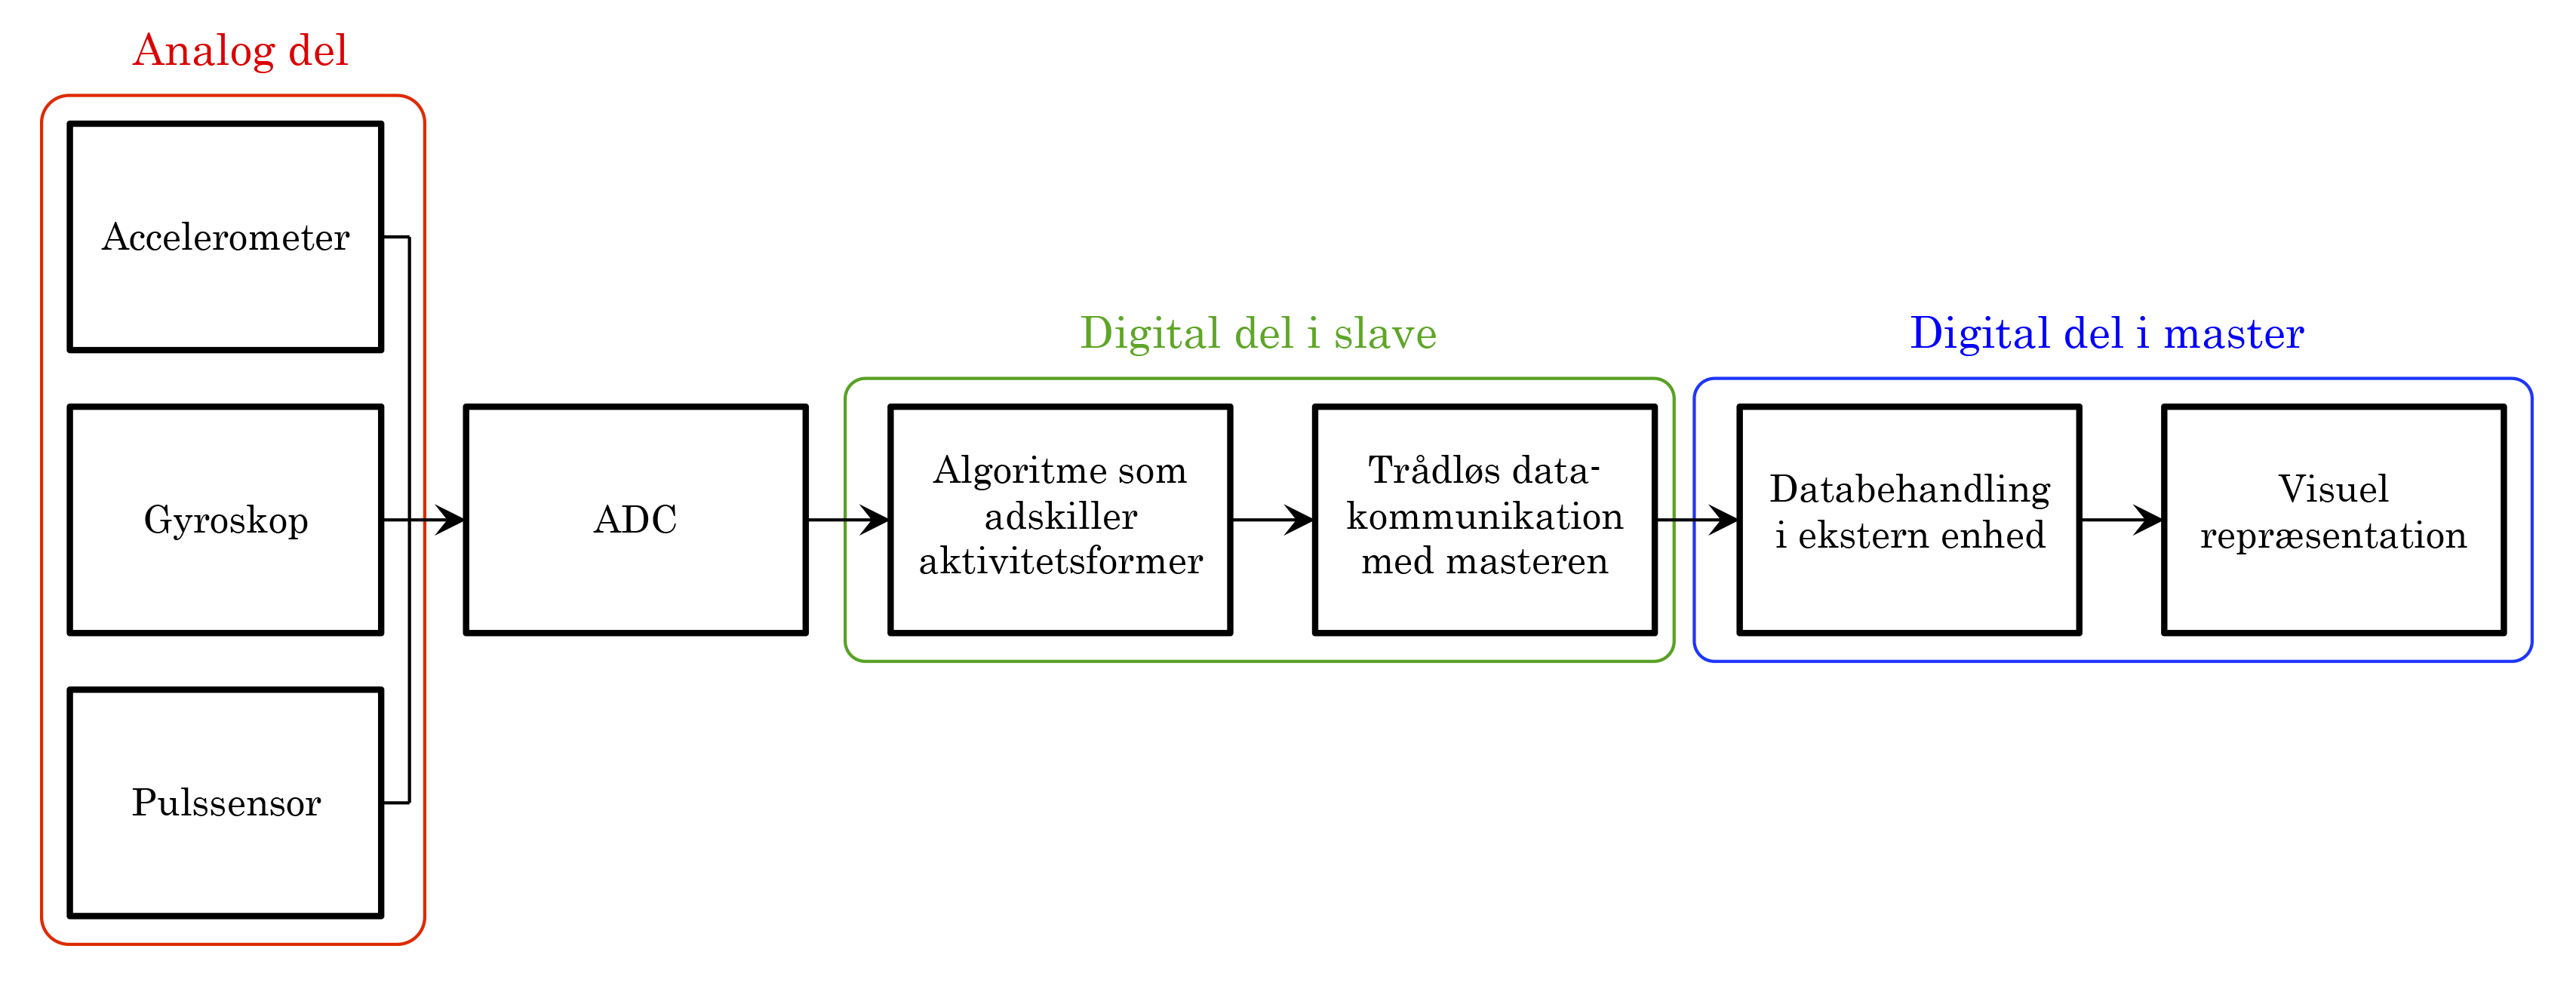
\includegraphics[scale=0.54]{figures/bProblemloesning/blokdiagram2.png}
 	\caption{På figuren ses blokdiagram for det samlede system, som opdeles i en analoge del og de to digitale dele. Den analoge del er omkranset med en rød firkant, slaven er omkranset med en grøn firkant og master er omkranset med en blå firkant.}
 	\label{fig:blokdiagram}
 \end{figure}